% =====================================================================
%  sc_body.tex -- shared content of the IEEE paper
%  "Skin Cancer Detection Using Deep Learning"
%  Sections:  I Introduction, II Literature Review, III Datasets,
%             IV Proposed Methodology, V Experimental Design,
%             VI Comparative Analysis of Algorithms, VII Discussion,
%             VIII Conclusion.
% =====================================================================

% =============================  TITLE  ================================
\title{Skin Cancer Detection Using Deep Learning: A Comparative Analysis
and a Multi-Model CNN--Transformer Ensemble with External Validation}

% ==== AUTHORS: team members and guide ==================================
%  (Add e-mail addresses here if the conference requires them.)
\ifCLASSOPTIONtwocolumn
  % larger author/affiliation fonts (IEEEtran style hooks)
  \makeatletter
  \def\@IEEEauthorblockNstyle{\normalfont\fontsize{13}{16}\selectfont}
  \def\@IEEEauthorblockAstyle{\normalfont\fontsize{10.5}{12.8}\selectfont}
  \makeatother
  \author{%
    \IEEEauthorblockN{Abhishek Patil, Jay Tripathi, Paras Shinkar, and Salman Sheikh}
    \IEEEauthorblockA{With the guidance of Dr.\ Bhakti Sonavane\\
                      Department of Computer Engineering\\
                      Shah \& Anchor Kutchhi Engineering College (Autonomous, Affiliated to University of Mumbai)\\
                      Mumbai, Maharashtra, India}}
\else
  \author{Abhishek~Patil,~Jay~Tripathi,~Paras~Shinkar,~and~Salman~Sheikh%
    \thanks{The authors are with the Department of Computer Engineering,
    Shah \& Anchor Kutchhi Engineering College (Autonomous, Affiliated to
    University of Mumbai), Mumbai, Maharashtra, India. This work was
    carried out with the guidance of Dr.~Bhakti Sonavane.}}
\fi

\maketitle

% ============================  ABSTRACT  =============================
\begin{abstract}
Early detection is the single most important factor in surviving skin
cancer, yet access to dermatologists is limited and visual diagnosis
of melanoma, basal cell carcinoma (BCC), and squamous cell carcinoma
(SCC) is error-prone even for experts. Deep learning has produced many
image classifiers for this task, but their published accuracies are
difficult to compare because studies differ in datasets, class
definitions, data splits, and metrics. This paper makes three
contributions. First, it presents a structured literature review of
40+ studies covering convolutional neural networks (CNNs), vision
transformers, hybrid and ensemble models, dermatology foundation
models, prospective clinical trials, explainability, and skin-tone
fairness. Second, it performs a comparative analysis of
published results for classical machine learning, VGG, ResNet,
DenseNet, MobileNet, EfficientNet, ConvNeXt, ViT, Swin, hybrid
CNN--transformer, ensemble, and foundation models on the HAM10000,
ISIC~2019, and ISIC~2020 benchmarks, and for U-Net-family segmentation
on ISIC~2018, separating random from patient-disjoint and official-test
protocols. The analysis shows that split leakage and dataset shift can
account for differences larger than those between architectures.
Third, guided by this evidence, it trains and evaluates a multi-model
ensemble that combines two CNNs (EfficientNetV2-S and ConvNeXt-T) and a
vision transformer (Swin-T) by temperature-calibrated soft voting. The
models are trained with focal loss on ISIC~2019 (25{,}331 dermoscopic
images, eight classes) using a de-duplicated, lesion-grouped split, and
are tested on a held-out internal set of 3{,}596 images and on the
external smartphone dataset PAD-UFES-20 (2{,}298 images). On the
internal test set, equal-weight soft voting achieved 77.95\% accuracy,
62.99\% balanced accuracy, a macro-AUC of 0.950, and 95.4\% malignant
sensitivity, exceeding the best single model (ConvNeXt-T: 76.89\%,
60.21\%, and 0.936); validation-weighted voting achieved 76.89\% accuracy
and 61.65\% balanced accuracy. On external smartphone images, accuracy
fell below 38\% for every model, quantifying the domain-shift problem
identified in the review, yet model combination still raised the
malignant-versus-benign AUC from at most 0.844 to 0.873.
\end{abstract}

\begin{IEEEkeywords}
Skin cancer, melanoma, deep learning, convolutional neural network,
vision transformer, ensemble learning, lesion segmentation, dermoscopy,
explainable AI, fairness.
\end{IEEEkeywords}

% ==========================  I. INTRODUCTION  ========================
\section{Introduction}
\IEEEPARstart{S}{kin} cancer is among the most frequently diagnosed
cancers worldwide. Melanoma causes most skin-cancer deaths, while the
keratinocyte cancers---BCC and SCC---are far more common and impose a
large treatment burden. Prognosis depends strongly on the stage at
which a lesion is found, so a tool that helps a non-specialist decide
quickly whether a lesion is suspicious has clear clinical value.

Visual assessment, with or without a dermatoscope, is the first step
in diagnosis. It is subjective, and its accuracy drops sharply outside
specialist clinics. Deep learning changed the field when a single CNN
matched board-certified dermatologists on biopsy-proven clinical
images~\cite{esteva2017derm}. Reader studies later reported
comparable or better performance than dermatologist
panels on dermoscopic images~\cite{haenssle2018man,brinker2019deep,
tschandl2019comparison}. Meta-analytic evidence now indicates that AI
reaches a pooled sensitivity of 87.0\% and specificity of 77.1\%, above
the corresponding values for clinicians as a group~\cite{salinas2024}.

Two problems still limit progress. \emph{First}, reported results are
hard to compare. Papers on the popular HAM10000 set~\cite{tschandl2018ham10000}
often split images at random, even though many lesions contribute
several near-identical photographs, so the same lesion can appear in
both training and test sets. When duplicates are removed from the ISIC
archives, the best area under the ROC curve (AUC) on the ISIC~2020 test
set falls to 0.80~\cite{cassidy2022isic}. The ISIC~2019 winning ensemble
lost about ten points of balanced accuracy between cross-validation and
the official hidden test set~\cite{gessert2020}. \emph{Second},
benchmark success has not reliably transferred to patients. In
prospective trials, AI tuned for high sensitivity often has low
specificity~\cite{marchetti2023,marsden2023}, and a smartphone
algorithm that led experimental benchmarks was inferior to specialists
in the clinic~\cite{menzies2023}. Public datasets also under-represent
darker skin~\cite{wen2022}, and model accuracy falls on these
patients~\cite{daneshjou2022ddi,groh2024}.

This paper addresses both problems. Its contributions are:
\begin{enumerate}
  \item A thematic \textbf{literature review} of more than 40 studies
        (Section~\ref{sec:lit}) that identifies six concrete research
        gaps.
  \item A curated \textbf{dataset analysis} (Section~\ref{sec:data})
        of eleven public skin-cancer datasets with verified image
        counts, class balance, and recommended roles, including the
        recent SLICE-3D and MILK10k collections.
  \item A \textbf{proposed methodology} (Section~\ref{sec:method}): a
        hybrid CNN--transformer ensemble with imbalance-aware training,
        probability calibration, and a sensitivity-driven referral
        rule, designed so that segmentation, metadata fusion, and
        explanations can be added as modules.
  \item A leakage-free \textbf{experimental design}
        (Section~\ref{sec:exp}) with de-duplication, lesion-grouped
        splitting, and an external test set.
  \item \textbf{Measured results} (Section~\ref{sec:results}) of the
        three backbones and their combination on internal and external
        data, with training curves, confusion matrices, ROC curves,
        confidence intervals, and a skin-type breakdown.
  \item A \textbf{comparative analysis of multiple algorithms}
        (Section~\ref{sec:compare}) that places published results and
        our own side by side, grouped by comparable protocol, together
        with graphs and a qualitative trade-off analysis.
\end{enumerate}

The remainder of the paper follows this order: literature review,
datasets, proposed methodology, experimental design, experimental
results, comparative analysis, discussion, and conclusion.

% ========================  II. LITERATURE REVIEW  ======================
\section{Literature Review}\label{sec:lit}
We searched IEEE Xplore, PubMed, Scopus, and arXiv for studies published
from 2015 to 2026 using combinations of the terms \emph{skin cancer},
\emph{melanoma}, \emph{skin lesion}, \emph{deep learning}, \emph{CNN},
\emph{transformer}, \emph{segmentation}, and \emph{dermoscopy}. We gave
priority to peer-reviewed journal papers, challenge reports, and
prospective clinical studies, and verified every bibliographic record
against its DOI. Earlier surveys~\cite{naqvi2023,hermosilla2024,naseri2025}
catalogue architectures but rarely compare them under a common
protocol; this review therefore emphasizes evaluation conditions
alongside reported numbers. Table~\ref{tab:lit} summarizes
representative studies; the paragraphs below organize the literature
into seven themes.

\subsection{Early Deep Learning and Reader Studies}
Esteva \emph{et al.}~\cite{esteva2017derm} fine-tuned an Inception
network on about 129{,}000 clinical images and reached
dermatologist-level performance on two binary tasks. Haenssle
\emph{et al.}~\cite{haenssle2018man} and Brinker
\emph{et al.}~\cite{brinker2019deep} compared CNNs with 58 and 157
dermatologists on dermoscopic melanoma images and found the networks
competitive or superior. In the ISIC~2018 reader study, the top three
algorithms averaged 25.43 correct answers per 30-image batch against
18.78 for experts, although their advantage shrank on images from
outside the training distribution~\cite{tschandl2019comparison}. These
studies established feasibility but used curated, retrospective images.

\subsection{Convolutional Neural Networks}
Transfer learning from ImageNet with standard CNNs---VGG~\cite{simonyan2015vgg},
ResNet~\cite{he2016resnet}, Inception~\cite{szegedy2016inception},
DenseNet~\cite{huang2017densenet}, Xception~\cite{chollet2017xception},
and MobileNet~\cite{sandler2018mobilenetv2}---is the most common
approach. On HAM10000, a MobileNet reached 83.1\% accuracy with a low
computational cost~\cite{chaturvedi2020mobilenet}. A comparison of
five CNNs found ResNeXt-101 best at 93.2\%~\cite{chaturvedi2020mtap},
and adding soft attention to InceptionResNetV2 raised accuracy to
93.4\%~\cite{datta2021soft}. Among EfficientNet variants~\cite{tan2019efficientnet},
B4 gave the best trade-off at 87.9\% accuracy~\cite{ali2022efficientnets}.
Shetty \emph{et al.}~\cite{shetty2022} showed that a small custom CNN
clearly outperforms classical baselines such as a support vector
machine (SVM) or random forest trained on the same data.

\subsection{Transformers, Hybrids, and Ensembles}
Vision transformers (ViT)~\cite{dosovitskiy2021vit} model long-range
relations between image patches. A modified ViT, SkinTrans, reported
94.3\% on HAM10000~\cite{xin2022skintrans}. On the harder eight-class
ISIC~2019 set, a Swin Transformer~\cite{liu2021swin} reached a
balanced accuracy of 82.3\%~\cite{ayas2023swin}, and an ensemble of
four ConvNeXt~\cite{liu2022convnext} models from the same group
raised the mean sensitivity to 84.2\%~\cite{baykal2024convnext}. Hybrid
designs pair a CNN, which captures local texture, with a transformer,
which captures global context. Nie \emph{et al.}~\cite{nie2023hybrid}
combined a ResNet stem with a ViT and focal loss, and Karthik
\emph{et al.}~\cite{karthik2024} fused Swin with a DenseNet attention
branch (94.2\% on HAM10000). MedFusionNet fuses ConvNeXt and ViT
features with attention~\cite{naeem2025}. Ensembles dominate challenge
leaderboards: Gessert \emph{et al.}~\cite{gessert2020} won ISIC~2019
with multi-resolution EfficientNets plus a metadata branch, and an
EfficientNet ensemble won the SIIM-ISIC~2020 melanoma
challenge~\cite{ha2020siim}.

\subsection{Lesion Segmentation}
Segmentation isolates the lesion from surrounding skin, hair, and
rulers. U-Net~\cite{ronneberger2015unet} remains the reference model;
attention gates~\cite{oktay2018attunet}, transformer encoders
(TransUNet)~\cite{chen2021transunet}, and channel-wise transformer skip
connections (UCTransNet)~\cite{wang2022uctransnet} are its main
successors. A survey of 177 papers~\cite{mirikharaji2023} identifies
artefacts and inconsistent annotation as the main open problems, and a
uniform re-evaluation of U-Net variants on ISIC~2018~\cite{azad2024unet}
provides directly comparable Dice scores (Section~\ref{sec:compare}).

\subsection{Class Imbalance and Synthetic Data}
Malignant lesions are the minority in almost every dataset
(Fig.~\ref{fig:prev}). Focal loss~\cite{lin2017focal} down-weights
easy examples. Under an identical backbone and split, it raised overall
accuracy from 74.2\% to 83.7\%~\cite{nie2023hybrid}. Generative
models provide an alternative route: an improved DCGAN reached high
accuracy on a binary ISIC~2017 task~\cite{behara2023}, synthetic
StyleGAN2 melanomas raised melanoma AUC from 0.925 to
0.945~\cite{lin2026}, and Stable Diffusion has also been used to
synthesize training lesions~\cite{farooq2024}. Evidence that synthetic
data helps on \emph{external} test sets is still limited.

\subsection{Explainability and Foundation Models}
A systematic review of explainable AI (XAI) for skin cancer found that
only 3 of 37 studies measured how explanations affect
clinicians~\cite{hauser2022}. Grad-CAM~\cite{selvaraju2017gradcam} is
the default tool, whereas dermoscopy-feature-based explanations
measurably increased dermatologists' trust~\cite{chanda2024}.
Foundation models are the newest trend. PanDerm was pretrained on more
than two million images and set the state of the art on 28
benchmarks~\cite{yan2025panderm}. MONET links images to medical
concepts for model auditing~\cite{kim2024monet}, and SkinGPT-4 adds a
conversational interface~\cite{zhou2024skingpt4}. These models are
powerful but computationally heavy. Lightweight alternatives such as
HI-MViT~\cite{ding2023} and SkinNet-14~\cite{almahmud2024} target
mobile deployment.

\subsection{Clinical Validation and Fairness}
Prospective studies give a more sober picture. The PROVE-AI study
reached 96.8\% sensitivity but only 37.4\% specificity~\cite{marchetti2023},
the DERM device detected all melanomas but had low specificity for
BCC and SCC~\cite{marsden2023}, and a multicentre German study found AI
more sensitive but less specific than dermatologists~\cite{heinlein2024}.
Only two of 272 primary-care studies used low-prevalence
data~\cite{jones2022}. Regarding equity, skin type is recorded for only
2.1\% of public images~\cite{wen2022}. Models degrade on the diverse DDI
set~\cite{daneshjou2022ddi}, and AI assistance can widen the accuracy
gap between light and dark skin~\cite{groh2024}.

\subsection{Research Gaps}
The review reveals six gaps that motivate this work:
\begin{itemize}[leftmargin=2.4em,labelsep=0.4em]
  \item[\textbf{G1}] \emph{Incomparable evaluation:} random image-level
        splits, varying class sets, and accuracy-only reporting inflate
        and obscure results~\cite{cassidy2022isic}.
  \item[\textbf{G2}] \emph{No external validation:} most architecture
        papers test only on data from the training
        distribution~\cite{karthik2024,naeem2025}.
  \item[\textbf{G3}] \emph{Imbalance and non-melanoma cancers:} BCC,
        SCC, and actinic keratosis receive less attention than
        melanoma~\cite{jones2022}.
  \item[\textbf{G4}] \emph{Skin-tone bias:} performance is rarely
        reported per Fitzpatrick type~\cite{wen2022,daneshjou2022ddi}.
  \item[\textbf{G5}] \emph{Limited explainability:} saliency maps are
        added but seldom evaluated~\cite{hauser2022}.
  \item[\textbf{G6}] \emph{Accuracy versus deployability:} strong
        foundation models are heavy, while light models lack external
        tests~\cite{yan2025panderm,ding2023}.
\end{itemize}

% -------- Literature summary table ------------------------------------
\begin{table*}[t]
\centering
\caption{Summary of reviewed literature on deep learning for skin cancer detection (results as reported by the authors).}
\label{tab:lit}
\renewcommand{\arraystretch}{1.15}
\scriptsize
\begin{tabularx}{\textwidth}{@{}L{2.4cm} c L{3.4cm} L{2.2cm} L{3.0cm} Y@{}}
\toprule
\textbf{Study} & \textbf{Year} & \textbf{Method} & \textbf{Dataset} & \textbf{Reported result} & \textbf{Limitation / gap} \\
\midrule
Esteva \emph{et al.}~\cite{esteva2017derm} & 2017 & Inception CNN, transfer learning & 129k clinical images & On par with 21 dermatologists & Private data; binary tasks \\
Tschandl \emph{et al.}~\cite{tschandl2019comparison} & 2019 & ISIC~2018 algorithms vs.\ 511 readers & ISIC~2018 test & Top-3 AI: 25.4 vs.\ 18.8 correct/30 & Advantage shrinks out of distribution \\
Chaturvedi \emph{et al.}~\cite{chaturvedi2020mtap} & 2020 & Five ImageNet CNNs & HAM10000 & Best (ResNeXt-101) 93.2\% acc. & Random split; no external test \\
Gessert \emph{et al.}~\cite{gessert2020} & 2020 & Multi-res.\ EfficientNet ensemble + metadata & ISIC~2019 & BA 74.2\% (CV), 63.6\% (official test) & Heavy ensemble; large CV--test gap \\
Datta \emph{et al.}~\cite{datta2021soft} & 2021 & InceptionResNetV2 + soft attention & HAM10000 & 93.4\% acc., AUC 0.984 & Resampled random split \\
Ali \emph{et al.}~\cite{ali2022efficientnets} & 2022 & EfficientNet B0--B7 & HAM10000 & B4: 87.9\% acc., F1 0.87 & Single dataset \\
Xin \emph{et al.}~\cite{xin2022skintrans} & 2022 & Improved ViT (SkinTrans) & HAM10000 & 94.3\% acc. & Split not detailed \\
Cassidy \emph{et al.}~\cite{cassidy2022isic} & 2022 & Duplicate audit of ISIC archives, 19 CNNs & ISIC 2016--2020 & Best AUC 0.80 after de-duplication & Shows benchmark inflation \\
Ayas~\cite{ayas2023swin} & 2023 & Swin Transformer & ISIC~2019 (8 cl.) & BA 82.3\%, spec.\ 97.9\% & Single model; no metadata \\
Nie \emph{et al.}~\cite{nie2023hybrid} & 2023 & ResNet + ViT hybrid, focal loss & ISIC~2018 & 89.5\% acc.; macro-F1 81.1\% & No external validation \\
Ding \emph{et al.}~\cite{ding2023} & 2023 & Lightweight MobileViT (HI-MViT) & ISIC~2018/2017, PH2 & 93.2\% acc., AUC 0.977 & No on-device latency reported \\
Marchetti \emph{et al.}~\cite{marchetti2023} & 2023 & Prospective open-source ensemble & 603 lesions, MSKCC & Sens.\ 96.8\%, spec.\ 37.4\% & Low specificity; 96\% white cohort \\
Menzies \emph{et al.}~\cite{menzies2023} & 2023 & Smartphone AI, prospective trial & 172 lesions, AU/AT & 7-class AI equal to specialists & ISIC AI inferior in clinic \\
Baykal Kablan \& Ayas~\cite{baykal2024convnext} & 2024 & ConvNeXt ensemble & ISIC~2019 (8 cl.) & Sens.\ 84.2\%, spec.\ 97.9\% & Same-lab split; no external test \\
Karthik \emph{et al.}~\cite{karthik2024} & 2024 & Swin + DenseNet attention hybrid & HAM10000 & 94.2\% acc., F1 96.6\% & One dataset only \\
Heinlein \emph{et al.}~\cite{heinlein2024} & 2024 & Prospective multicentre AI & 8 German hospitals & BA 0.798 vs.\ 0.781 (dermatol.) & Specificity 0.67 vs.\ 0.83 \\
Groh \emph{et al.}~\cite{groh2024} & 2024 & AI-assisted diagnosis experiment & 364 images, 848 physicians & AI aid $>$33\% accuracy gain & Widens skin-tone gap \\
Salinas \emph{et al.}~\cite{salinas2024} & 2024 & Meta-analysis, AI vs.\ clinicians & 53 studies & AI sens.\ 87.0\%, spec.\ 77.1\% & Mostly retrospective \\
Chanda \emph{et al.}~\cite{chanda2024} & 2024 & Dermoscopy-feature XAI & Reader study & Higher clinician trust & Melanoma vs.\ nevus only \\
Yan \emph{et al.}~\cite{yan2025panderm} & 2025 & PanDerm foundation model & 2M+ images, 28 tasks & SOTA on 28 benchmarks & Very high compute cost \\
Naeem \emph{et al.}~\cite{naeem2025} & 2025 & ConvNeXt + ViT attention fusion & HAM10000, ISIC~2019 & 98.8\% / 97.9\% acc. & Benchmark-only evaluation \\
Lin \emph{et al.}~\cite{lin2026} & 2026 & StyleGAN2 synthetic melanoma & ISIC~2018/2020 & Melanoma AUC 0.925$\rightarrow$0.945 & Melanoma class only \\
\bottomrule
\end{tabularx}
\end{table*}

% ============================  III. DATASETS  ==========================
\section{Datasets}\label{sec:data}
Choosing datasets is as important as choosing an architecture. We
reviewed eleven public datasets (Table~\ref{tab:data}). The experiments
in this paper use the \textbf{two} that best fit the task: ISIC~2019 for
training and internal testing, and PAD-UFES-20 as an external test set.
Together they cover all three major skin cancers, two imaging
modalities, and two continents, without overlapping images.

\textbf{Training and internal test data: ISIC~2019.} ISIC~2019 is the
largest multi-class dermoscopic set, with 25{,}331 training images in
eight classes, including melanoma (MEL), BCC, SCC, and actinic keratosis
(AK) (Fig.~\ref{fig:isic19}). It already contains
HAM10000~\cite{tschandl2018ham10000} and
BCN20000~\cite{hernandez2024bcn20000}, so these are \emph{not} added
again. We split it into training (18{,}076 images), validation (3{,}659),
and internal test (3{,}596) sets as described in
Section~\ref{sec:exp}.

\textbf{External test data: PAD-UFES-20.}
PAD-UFES-20~\cite{pacheco2020padufes20} contains 2{,}298 smartphone
images collected in Brazil, with biopsy-proven cancers and the
patient's Fitzpatrick skin type. It is never used for training. Its six
diagnoses map onto ISIC~2019 classes (ACK$\rightarrow$AK,
NEV$\rightarrow$NV, SEK$\rightarrow$BKL; BCC, SCC, and MEL unchanged),
so it tests whether a dermoscopy-trained model transfers to ordinary
phone photographs.

\textbf{Datasets for the next stage.} ISIC~2020~\cite{rotemberg2021isic2020}
(33{,}126 images, 1.8\% melanoma) can add realistic-prevalence melanoma
training data. MILK10k~\cite{tschandl2026milk10k}, the ISIC~2025
benchmark (5{,}240 lesions, 11 classes), and DDI~\cite{daneshjou2022ddi},
which is balanced across Fitzpatrick groups, are planned as further
external and fairness test sets. ISIC~2018 Task~1~\cite{codella2019isic2018}
and PH2~\cite{mendonca2013ph2} provide lesion masks for the segmentation
module. SLICE-3D~\cite{kurtansky2024slice3d} (401{,}059 crops, 0.1\%
malignant), the basis of the ISIC~2024 triage challenge~\cite{kurtansky2025},
is reserved for future triage experiments. Derm7pt~\cite{kawahara2019derm7pt},
which annotates the seven-point dermoscopic checklist, is a candidate
for evaluating concept-level explanations. Fig.~\ref{fig:prev} shows
how strongly malignant prevalence varies between datasets. This
variation is a key reason why a single accuracy number is misleading.

\begin{table*}[t]
\centering
\caption{Public skin-cancer datasets reviewed (counts verified against official label files or data papers) and their role in this work.}
\label{tab:data}
\renewcommand{\arraystretch}{1.15}
\scriptsize
\begin{tabularx}{\textwidth}{@{}l c r l L{4.2cm} l Y@{}}
\toprule
\textbf{Dataset} & \textbf{Year} & \textbf{Images} & \textbf{Modality} & \textbf{Classes (malignant in bold)} & \textbf{Metadata} & \textbf{Role in this work} \\
\midrule
HAM10000~\cite{tschandl2018ham10000} & 2018 & 10{,}015 & Dermoscopic & 7: \textbf{MEL}, \textbf{BCC}, \textbf{AKIEC}, NV, BKL, DF, VASC & Age, sex, site & Included via ISIC~2019 \\
ISIC~2017~\cite{codella2018isic2017} & 2017 & 2{,}750 & Dermoscopic & 3: \textbf{MEL}, SK, NV & Age, sex & Background / literature \\
ISIC~2018~\cite{codella2019isic2018} & 2018 & 2{,}594 (T1) & Dermoscopic & Masks (Task~1); 7 classes (Task~3) & -- & Future: segmentation \\
ISIC~2019~\cite{gessert2020} & 2019 & 25{,}331 & Dermoscopic & 8: \textbf{MEL}, \textbf{BCC}, \textbf{SCC}, \textbf{AK}, NV, BKL, DF, VASC & Age, sex, site & \textbf{Used: training + internal test} \\
BCN20000~\cite{hernandez2024bcn20000} & 2024 & 18{,}946 & Dermoscopic & 8 (as ISIC~2019) + OOD & Age, sex, site & Included via ISIC~2019 \\
ISIC~2020~\cite{rotemberg2021isic2020} & 2020 & 33{,}126 & Dermoscopic & Binary: \textbf{MEL} (1.8\%) vs.\ benign & Patient ID, age, sex, site & Future: melanoma training \\
SLICE-3D~\cite{kurtansky2024slice3d} & 2024 & 401{,}059 & 3D-TBP crops & Binary: \textbf{malignant} (0.1\%) vs.\ benign & Age, sex, site, TBP features & Future triage work \\
MILK10k~\cite{tschandl2026milk10k} & 2026 & 10{,}480 & Clinical + dermoscopic & 11 incl.\ \textbf{BCC}, \textbf{SCC}, \textbf{MEL}, \textbf{AKIEC} & Age, sex, site, skin tone & Future: external test \\
PH2~\cite{mendonca2013ph2} & 2013 & 200 & Dermoscopic & 3: \textbf{MEL}, atypical NV, common NV & Masks, criteria & Future: segmentation test \\
PAD-UFES-20~\cite{pacheco2020padufes20} & 2020 & 2{,}298 & Smartphone & 6: \textbf{BCC}, \textbf{SCC}, \textbf{MEL}, ACK, SEK, NEV & 21 fields incl.\ Fitzpatrick & \textbf{Used: external test} \\
Fitzpatrick 17k~\cite{groh2021fitzpatrick17k} & 2021 & 16{,}577 & Clinical & 114 conditions; 3-way incl.\ \textbf{malignant} & Fitzpatrick I--VI & Optional fairness analysis \\
DDI~\cite{daneshjou2022ddi} & 2022 & 656 & Clinical & Binary: \textbf{malignant} vs.\ benign & Fitzpatrick groups & Future: fairness test \\
\bottomrule
\end{tabularx}
\end{table*}

\begin{figure}[t]
\centering
\begin{tikzpicture}
\begin{axis}[hcaxis,
  width=\chartw,height=\charth,
  ybar, bar width=9pt,
  symbolic x coords={NV,MEL,BCC,BKL,AK,SCC,VASC,DF},
  xtick={NV,MEL,BCC,BKL,AK,SCC,VASC,DF}, x tick label style={font=\scriptsize},
  bar shift=0pt,
  ylabel={Number of images},
  ymin=0,ymax=14500, nodes near coords,
  every node near coord/.append style={font=\tiny},
  scaled y ticks=false,
  yticklabel style={/pgf/number format/fixed,/pgf/number format/1000 sep={,}},
  enlarge x limits=0.08]
\addplot[fill=hcBlue,draw=hcBlue!60] coordinates {(NV,12875)(BKL,2624)(VASC,253)(DF,239)};
\addplot[fill=hcRed,draw=hcRed!60] coordinates {(MEL,4522)(BCC,3323)(AK,867)(SCC,628)};
\legend{Benign,Malignant / pre-malignant}
\end{axis}
\end{tikzpicture}
\caption{Class distribution of the ISIC~2019 training set (25{,}331
images). The largest class (NV) is 54$\times$ the smallest (DF), and
SCC has only 628 images, which motivates imbalance-aware training.}
\label{fig:isic19}
\end{figure}

\begin{figure}[t]
\centering
\begin{tikzpicture}
\begin{axis}[hcaxis,
  width=\barchartw,height=\charth,
  xbar, bar width=7pt,
  ytick={1,2,3,4,5,6,7},
  yticklabels={SLICE-3D,ISIC 2020,Fitzpatrick 17k,HAM10000,DDI,ISIC 2019,PAD-UFES-20},
  y tick label style={font=\scriptsize},
  xlabel={Malignant share (\%)},
  xmin=0,xmax=60, nodes near coords,
  every node near coord/.append style={font=\tiny},
  enlarge y limits=0.1]
\addplot[fill=hcOrange,draw=hcOrange!60] coordinates {
 (0.1,1)(1.8,2)(13.7,3)(19.5,4)(26.1,5)(36.9,6)(47.4,7)};
\end{axis}
\end{tikzpicture}
\caption{Share of malignant images per dataset, computed from the
official label files (HAM10000 and ISIC~2019 include the
AKIEC/AK class; PAD-UFES-20 counts BCC, SCC, and MEL). Prevalence ranges
from 0.1\% to 47\%, so accuracy alone is not comparable across
datasets.}
\label{fig:prev}
\end{figure}

% ======================  IV. PROPOSED METHODOLOGY  =====================
\section{Proposed Methodology}\label{sec:method}
The proposed system, shown in Fig.~\ref{fig:pipeline}, answers the gaps
of Section~\ref{sec:lit} with evidence-backed components rather than an
untested new architecture. It contains six stages: preprocessing,
lesion segmentation, a three-backbone hybrid ensemble, metadata fusion,
calibrated decision making, and explanation. Section~\ref{sec:impl}
states exactly which of these stages are evaluated in the experiments
of this paper.

\ifCLASSOPTIONtwocolumn\begin{figure*}[t]\else\begin{figure}[t]\fi
\centering
\begin{tikzpicture}[
  font=\scriptsize, node distance=3mm and 3.2mm,
  blk/.style={draw=hcBlue!70,fill=hcBlue!6,rounded corners=2pt,
     minimum height=8mm,minimum width=14mm,align=center},
  bb/.style={draw=hcPurple!70,fill=hcPurple!8,rounded corners=2pt,
     minimum height=6mm,minimum width=20mm,align=center},
  data/.style={draw=hcTeal!75,fill=hcTeal!8,rounded corners=2pt,
     minimum height=8mm,minimum width=14mm,align=center},
  outbox/.style={draw=hcOrange!80,fill=hcOrange!8,rounded corners=2pt,
     minimum height=6.5mm,minimum width=18mm,align=center},
  flow/.style={-{Latex[length=1.8mm]},draw=hcGray,thick}]
\node[data] (img) {Input\\image};
\node[blk,right=of img] (pre) {Hair removal,\\colour\\constancy};
\node[blk,right=of pre] (seg) {Attention\\U-Net};
\node[blk,right=of seg] (roi) {ROI crop +\\augmentation};
\node[bb,right=6mm of roi,yshift=7.5mm] (b1) {EfficientNetV2-S};
\node[bb,below=2mm of b1] (b2) {ConvNeXt-T};
\node[bb,below=2mm of b2] (b3) {Swin-T};
\node[data,below=9mm of roi] (meta) {Metadata\\age, sex, site};
\node[blk,right=6mm of meta,yshift=-3mm] (mlp) {MLP\\encoder};
\node[blk,right=6mm of b2] (fuse) {Feature\\fusion +\\heads};
\node[blk,right=4mm of fuse] (ens) {Weighted\\soft vote,\\TTA, temp.};
\node[outbox,right=4mm of ens,yshift=7.5mm] (pred) {Class + $P_{mal}$};
\node[outbox,below=2mm of pred] (cam) {Grad-CAM map};
\node[outbox,below=2mm of cam] (ref) {Refer / monitor};
\draw[flow] (img)--(pre); \draw[flow] (pre)--(seg); \draw[flow] (seg)--(roi);
\draw[flow] (roi.east)--(b1.west); \draw[flow] (roi.east)--(b2.west); \draw[flow] (roi.east)--(b3.west);
\draw[flow] (b1.east)--(fuse.west); \draw[flow] (b2.east)--(fuse.west); \draw[flow] (b3.east)--(fuse.west);
\draw[flow] (meta)--(mlp.west|-meta);
\draw[flow] (mlp.east) -| (fuse.south);
\draw[flow] (fuse)--(ens);
\draw[flow] (ens.east)--(pred.west); \draw[flow] (ens.east)--(cam.west); \draw[flow] (ens.east)--(ref.west);
\end{tikzpicture}
\caption{Proposed hybrid ensemble framework. The lesion is classified by
three complementary backbones (two CNNs, one transformer) whose
calibrated outputs are combined by soft voting into class
probabilities and a referral recommendation. The experiments in
Section~\ref{sec:results} evaluate the three-backbone ensemble with
calibration and the referral rule on whole images; segmentation,
metadata fusion, and Grad-CAM are modules for the next stage.}
\label{fig:pipeline}
\ifCLASSOPTIONtwocolumn\end{figure*}\else\end{figure}\fi

\subsection{Implemented Configuration}\label{sec:impl}
The experiments reported in Section~\ref{sec:results} evaluate the core
of the framework: the three-backbone ensemble
(Section~\ref{sec:m_backbones}), imbalance-aware training
(Section~\ref{sec:m_imb}), and the calibrated soft vote with its
referral rule (Section~\ref{sec:m_ens}), applied to whole lesion
images. Lesion segmentation, metadata fusion, and Grad-CAM
(Sections~\ref{sec:m_seg}, \ref{sec:m_meta}, and \ref{sec:m_xai}) are
designed as plug-in modules for the next stage, so that the
contribution of each can later be measured against the baseline
reported here.

\subsection{Preprocessing}
All images are first resized so that their shorter side is 256 pixels.
During training, a random resized crop (scale 0.5--1.0) of
$224\times224$ pixels is taken; at test time the image is resized to
224 pixels and centre-cropped. Hair and ruler artefact removal
(morphological black-hat filtering with inpainting) and Shades-of-Gray
colour constancy belong to the full framework but were not applied in
the reported experiments.

\subsection{Lesion Segmentation (Next Stage)}\label{sec:m_seg}
An attention U-Net~\cite{oktay2018attunet} with an EfficientNet encoder
will be trained on ISIC~2018 Task~1. Attention gates in the skip
connections suppress background skin. Training minimizes the sum of
the Dice loss and binary cross-entropy:
\begin{equation}
\begin{split}
\mathcal{L}_{seg} ={}& 1-\frac{2\sum_i p_i g_i+\epsilon}{\sum_i p_i+\sum_i g_i+\epsilon}\\
 &-\frac{1}{N}\sum_i\big[g_i\log p_i+(1-g_i)\log(1-p_i)\big],
\end{split}
\label{eq:seg}
\end{equation}
where $p_i$ is the predicted foreground probability and $g_i$ the
ground-truth label of pixel $i$. The mask defines a region of interest
(ROI) that is cropped with a 15\% margin so that the classifier sees the
lesion border and some surrounding skin. Panel~D of the comparative
analysis (Table~\ref{tab:compare}) supports the attention U-Net as the
most accurate U-Net variant that remains light enough to train on a
single GPU.

\subsection{Hybrid Backbone Ensemble}\label{sec:m_backbones}
Three backbones pretrained on ImageNet-21k (public \texttt{timm}
weights) are fine-tuned with a new eight-class head:
\begin{itemize}
  \item \textbf{EfficientNetV2-S}~\cite{tan2021efficientnetv2}: compound-scaled
        CNN; EfficientNets are the most successful family in ISIC
        challenges~\cite{gessert2020,ha2020siim}.
  \item \textbf{ConvNeXt-T}~\cite{liu2022convnext}: a modernized CNN
        whose ensemble gave the best reported ISIC~2019
        sensitivity~\cite{baykal2024convnext}.
  \item \textbf{Swin-T}~\cite{liu2021swin}: a hierarchical
        transformer that captures global context and makes errors that
        differ from those of the CNNs~\cite{ayas2023swin}.
\end{itemize}
Diversity is deliberate: combining local (CNN) and global
(transformer) features consistently improves results over either
alone~\cite{nie2023hybrid,karthik2024}.

\subsection{Metadata Fusion (Next Stage)}\label{sec:m_meta}
Age, sex, and anatomical site are available in ISIC~2019/2020,
MILK10k, and PAD-UFES-20. They will be one-hot or min--max encoded and
passed through a two-layer perceptron (MLP) $g(\cdot)$. For backbone
$m$ with pooled image features $\mathbf{f}_m$, the fused representation
is
\begin{equation}
\mathbf{z}_m = \big[\,\mathbf{f}_m \,\Vert\, g(\mathbf{x}_{meta})\,\big],\qquad
\mathbf{p}_m = \mathrm{softmax}(W_m\mathbf{z}_m+\mathbf{b}_m),
\end{equation}
where $\Vert$ denotes concatenation. Metadata gave consistent gains in
the ISIC~2019 winning solution~\cite{gessert2020}.

\subsection{Imbalance-Aware Training}\label{sec:m_imb}
Each backbone is trained with the multi-class focal loss~\cite{lin2017focal}
\begin{equation}
\mathcal{L}_{FL} = -\sum_{c=1}^{C}\alpha_c\,(1-p_{c})^{\gamma}\,y_c\log p_{c},
\label{eq:focal}
\end{equation}
where $y_c$ is the one-hot label, $p_c$ the predicted probability,
$\gamma=2$ the focusing parameter, and $\alpha_c\propto 1/\sqrt{n_c}$ a
class weight computed from the number of training images $n_c$ of class
$c$ and normalized to mean one. Augmentation (horizontal and vertical
flips, random rotation up to $45^\circ$, random resized crops, and
colour jitter) further protects the minority classes SCC, AK, and DF;
no re-sampling is used.

\subsection{Calibrated Ensemble and Decision Rule}\label{sec:m_ens}
The final probability vector is a weighted soft vote over the $M=3$
models with test-time augmentation (TTA) over $T=4$ views (original,
horizontal flip, vertical flip, and both):
\begin{equation}
\hat{\mathbf{p}} = \sum_{m=1}^{M} w_m\,
\mathrm{softmax}\!\Big(\frac{1}{T\tau_m}\sum_{t=1}^{T}\mathbf{s}_{m,t}\Big),\qquad \sum_m w_m = 1,
\label{eq:ens}
\end{equation}
where $\mathbf{s}_{m,t}$ are the logits of model $m$ on view $t$ and
$\tau_m$ is a temperature fitted per model by minimizing the validation
negative log-likelihood. We evaluate two weightings: \emph{equal}
weights ($w_m=1/3$) and \emph{learned} weights chosen by a grid search
(step 0.05) that maximizes validation balanced accuracy. Calibration
makes the malignancy probability
$P_{mal}=\sum_{c\in\{\mathrm{MEL,BCC,SCC,AK}\}}\hat{p}_c$ meaningful.
A lesion is flagged for referral when $P_{mal}$ exceeds a threshold
$\theta$ selected on the validation set as the largest value that still
gives at least 95\% malignant sensitivity. This operating point is chosen
explicitly because prospective studies show that specificity collapses
when it is left implicit~\cite{marchetti2023,marsden2023}.

\subsection{Explainability (Next Stage)}\label{sec:m_xai}
For the predicted class $c$, Grad-CAM~\cite{selvaraju2017gradcam}
computes channel weights and a localization map from the last
convolutional (or last Swin stage) feature maps $A^k$:
\begin{equation}
\alpha_k^c=\frac{1}{Z}\sum_{i}\sum_{j}\frac{\partial y^c}{\partial A^k_{ij}},\qquad
L^c_{\text{Grad-CAM}}=\mathrm{ReLU}\Big(\sum_k\alpha_k^c A^k\Big).
\end{equation}
The ensemble map is the weighted average of the three model maps, and
explanation quality will be quantified by the fraction of heatmap
energy that falls inside the segmentation mask.

\subsection{Training Procedure}
Algorithm~\ref{alg:train} summarizes training, and
Table~\ref{tab:hyper} lists the settings used. Each backbone was trained
on a single NVIDIA GeForce RTX 3060 Laptop GPU (6\,GB) with bfloat16
mixed precision; peak GPU memory stayed below 3\,GB. Training took 43,
49, and 36 minutes for EfficientNetV2-S, ConvNeXt-T, and Swin-T,
respectively (Swin-T stopped early after 11 epochs).

\begin{algorithm}[t]
\caption{Training and evaluation of the hybrid ensemble}
\label{alg:train}
\footnotesize
\begin{algorithmic}[1]
\Require ISIC 2019 images and labels; PAD-UFES-20 (external)
\State Resize images (shorter side 256 px); compute a 64-bit image hash
\State Group images by lesion ID and identical hash
\State Stratified group split into train / val / test ($\approx$71/14/14\%)
\For{backbone $m \in$ \{EffNetV2-S, ConvNeXt-T, Swin-T\}}
  \State Initialize from ImageNet-21k weights; new 8-class head
  \For{epoch $=1$ to $20$}
    \State Train with focal loss (Eq.~\ref{eq:focal}), AdamW, warm-up + cosine
    \State Keep checkpoint with best validation balanced accuracy
    \State Stop if no improvement for 6 epochs
  \EndFor
\EndFor
\State Fit temperature $\tau_m$ per model on the validation set
\State Choose weights $w_m$ (equal, or grid search on validation; Eq.~\ref{eq:ens})
\State Choose threshold $\theta$ for $\geq95\%$ malignant sensitivity on validation
\State \Return evaluate once on the internal test set and on PAD-UFES-20
\end{algorithmic}
\end{algorithm}

\begin{table}[t]
\centering
\caption{Training configuration used in the experiments.}
\label{tab:hyper}
\renewcommand{\arraystretch}{1.12}
\footnotesize
\begin{tabularx}{\columnwidth}{@{}l Y@{}}
\toprule
\textbf{Setting} & \textbf{Value} \\
\midrule
Input size & $224\times224$ (random resized crop, scale 0.5--1.0) \\
Optimizer & AdamW, weight decay 0.05, gradient clipping 1.0 \\
Learning rate & $10^{-4}$ backbone, $10^{-3}$ head; 1-epoch warm-up, cosine decay \\
Epochs / batch & up to 20 (early stopping, patience 6) / 32 \\
Loss & Focal, $\gamma=2$, $\alpha_c\propto 1/\sqrt{n_c}$ \\
Regularization & Stochastic depth 0.1 \\
Augmentation & H/V flip, rotation $\leq45^\circ$, resized crop, colour jitter \\
Data split & Lesion-grouped, stratified: 18{,}076 / 3{,}659 / 3{,}596 \\
TTA / ensemble & 4 flips; temperature scaling; soft vote \\
Hardware & RTX 3060 Laptop GPU (6\,GB), bfloat16 \\
Framework & PyTorch 2.10, \texttt{timm} 1.0 \\
\bottomrule
\end{tabularx}
\end{table}

% ======================  V. EXPERIMENTAL DESIGN  =======================
\section{Experimental Design and Evaluation Metrics}\label{sec:exp}
\subsection{Leakage-Free Protocol}
Following the recommendations in~\cite{cassidy2022isic}, every image
receives a 64-bit difference hash. Images that share a lesion
identifier or an identical hash are merged into one group; the hash
step merged 344 groups that would otherwise have been split apart.
ISIC~2019 is then divided with stratified group $k$-fold sampling into
training (18{,}076 images), validation (3{,}659), and internal test
(3{,}596) sets, with no group shared between sets. The validation set is
used for checkpoint selection, temperatures, ensemble weights, and the
referral threshold; the internal test set and PAD-UFES-20 are used only
once, after all choices were frozen. For PAD-UFES-20, the eight-class
output is restricted to its six classes and renormalized.

\subsection{Metrics}
With $TP_c$, $FN_c$, $FP_c$, and $TN_c$ the per-class confusion counts
over $C$ classes, we report
\begin{align}
\mathrm{Acc} &= \frac{\sum_c TP_c}{N},\qquad
\mathrm{BA} = \frac{1}{C}\sum_{c=1}^{C}\frac{TP_c}{TP_c+FN_c},\\
\mathrm{Prec}_c &= \frac{TP_c}{TP_c+FP_c},\qquad
\mathrm{Spec}_c = \frac{TN_c}{TN_c+FP_c},\\
F1_c &= \frac{2TP_c}{2TP_c+FP_c+FN_c},
\end{align}
where $N$ is the number of test images. We report accuracy, balanced
accuracy, macro-averaged precision and F1, macro one-vs-rest ROC-AUC,
malignant-versus-benign AUC, sensitivity and specificity at threshold
$\theta$, and the expected calibration error (ECE). Balanced accuracy
(BA) is the primary metric because it is the official ISIC~2019 metric
and is insensitive to class prevalence. 95\% confidence intervals are
obtained with 1{,}000 bootstrap resamples of the test images.

\subsection{Fairness and Robustness Analysis}
PAD-UFES-20 records the Fitzpatrick skin type for 1{,}494 of its images.
External results are therefore also reported for Fitzpatrick groups
I--II, III--IV, and V--VI. Robustness is measured as the drop from the
internal to the external test set. DDI will extend the skin-tone
analysis in the next stage.

\subsection{Ablation}
To measure the contribution of model combination, every subset of the
three backbones is evaluated with equal-weight soft voting
(Table~\ref{tab:ablation}). Comparisons with further baselines
(ResNet-50, DenseNet-121, MobileNetV2, and a DINOv2 linear
probe~\cite{yan2025panderm}) are planned.

% ======================  VI. EXPERIMENTAL RESULTS  =====================
\section{Experimental Results}\label{sec:results}
All numbers in this section were measured by us on held-out data that
was not used for training or model selection.

\subsection{Training Behaviour}
Fig.~\ref{fig:curves} shows the training curves. Validation balanced
accuracy rose quickly during the first five epochs and then fluctuated
between about 58\% and 65\%. The training loss kept falling while the
validation loss began to rise after epoch 5--8, so checkpoint selection
on validation balanced accuracy was essential to limit overfitting. The
best validation balanced accuracies were 64.16\% (EfficientNetV2-S,
epoch 19), 64.61\% (ConvNeXt-T, epoch 17), and 63.05\% (Swin-T, epoch 5;
early-stopped at epoch 11).

\ifCLASSOPTIONtwocolumn\begin{figure*}[t]\else\begin{figure}[t]\fi
\centering
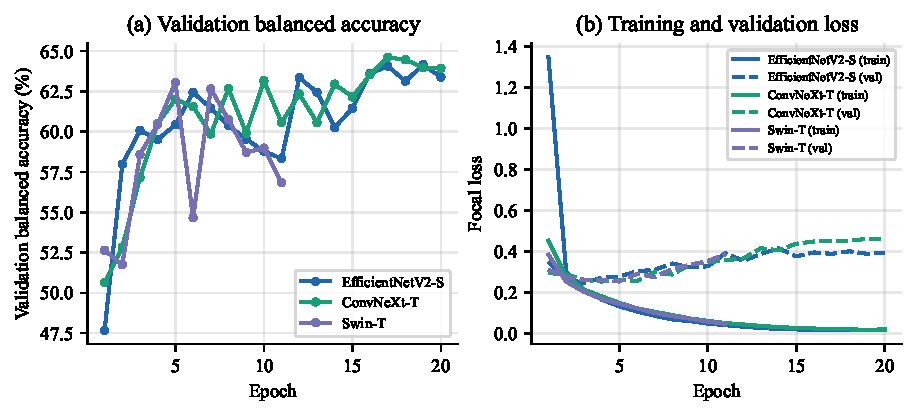
\includegraphics[width=\ifCLASSOPTIONtwocolumn0.82\textwidth\else\linewidth\fi]{figures/fig_training_curves.pdf}
\caption{Measured training curves of the three backbones on ISIC~2019:
(a) validation balanced accuracy per epoch and (b) training (solid) and
validation (dashed) focal loss.}
\label{fig:curves}
\ifCLASSOPTIONtwocolumn\end{figure*}\else\end{figure}\fi

\subsection{Internal Test Set (ISIC~2019)}
Table~\ref{tab:res_internal} and Fig.~\ref{fig:comparison}(a) report the
results on the 3{,}596 held-out ISIC~2019 images. Among the single
models, ConvNeXt-T was best (76.89\% accuracy, 60.21\% balanced
accuracy), followed by EfficientNetV2-S (75.19\%, 58.88\%) and Swin-T
(73.08\%, 57.80\%). Combining the three models with equal weights gave
the best result on every main metric: \textbf{77.95\% accuracy}
(95\% CI 76.6--79.3; 2{,}803 of 3{,}596 images correct),
\textbf{62.99\% balanced accuracy} (CI 59.5--66.4), \textbf{68.67\%
macro-precision}, 64.79\% macro-F1, and a macro-AUC of 0.950. The
validation-weighted ensemble (weights 0.60, 0.15, and 0.25 for
EfficientNetV2-S, ConvNeXt-T, and Swin-T) reached 76.89\% accuracy and
61.65\% balanced accuracy. That it did not beat equal weighting
indicates that the weight search slightly overfitted the validation
set. At the referral threshold, the equal-weight ensemble detected
95.4\% of malignant or pre-malignant lesions at 69.9\% specificity. This
is a higher specificity than any single model achieved at a similar
sensitivity (58.1--64.8\%), so it would send fewer harmless lesions for
referral.

\begin{table}[t]
\centering
\caption{Measured results on the internal test set (ISIC~2019, 3{,}596
lesion-disjoint images, 8 classes). Acc., BA, macro-precision (Prec.),
macro-F1, and malignant sensitivity/specificity in \%.}
\label{tab:res_internal}
\renewcommand{\arraystretch}{1.15}
\scriptsize
\setlength{\tabcolsep}{3pt}
\begin{tabular}{@{}l c c c c c c c@{}}
\toprule
\textbf{Model} & \textbf{Acc.} & \textbf{BA} & \textbf{Prec.} & \textbf{F1} & \textbf{AUC} & \textbf{Sens.} & \textbf{Spec.} \\
\midrule
EfficientNetV2-S & 75.19 & 58.88 & 61.66 & 59.32 & 0.943 & 94.5 & 64.8 \\
ConvNeXt-T & 76.89 & 60.21 & 67.95 & 62.68 & 0.936 & 97.1 & 58.1 \\
Swin-T & 73.08 & 57.80 & 57.84 & 56.47 & 0.935 & 94.1 & 61.3 \\
\textbf{Ensemble (equal)} & \textbf{77.95} & \textbf{62.99} & \textbf{68.67} & \textbf{64.79} & \textbf{0.950} & 95.4 & \textbf{69.9} \\
Ensemble (learned) & 76.89 & 61.65 & 65.82 & 62.47 & 0.950 & 94.5 & 69.2 \\
\bottomrule
\end{tabular}
\end{table}

\ifCLASSOPTIONtwocolumn\begin{figure*}[t]\else\begin{figure}[t]\fi
\centering
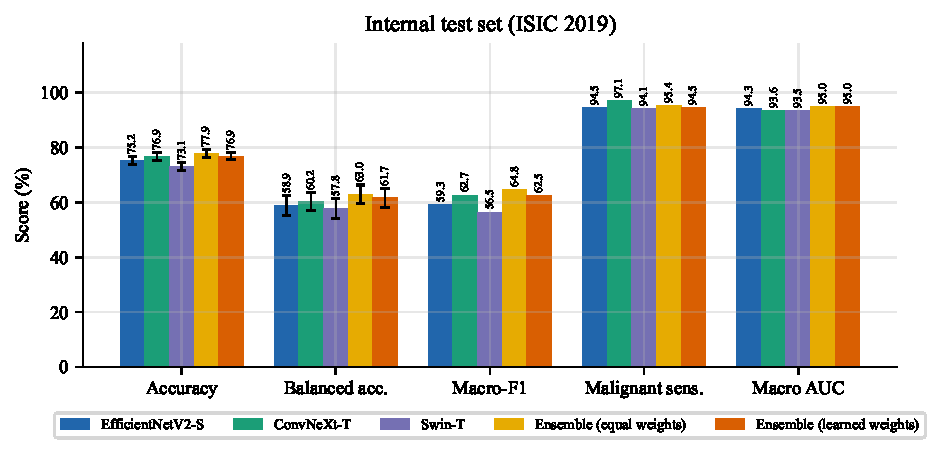
\includegraphics[width=\ifCLASSOPTIONtwocolumn0.80\textwidth\else\linewidth\fi]{figures/fig_model_comparison.pdf}\\[2pt]
{\footnotesize (a) Internal test set (ISIC~2019)}\\[4pt]
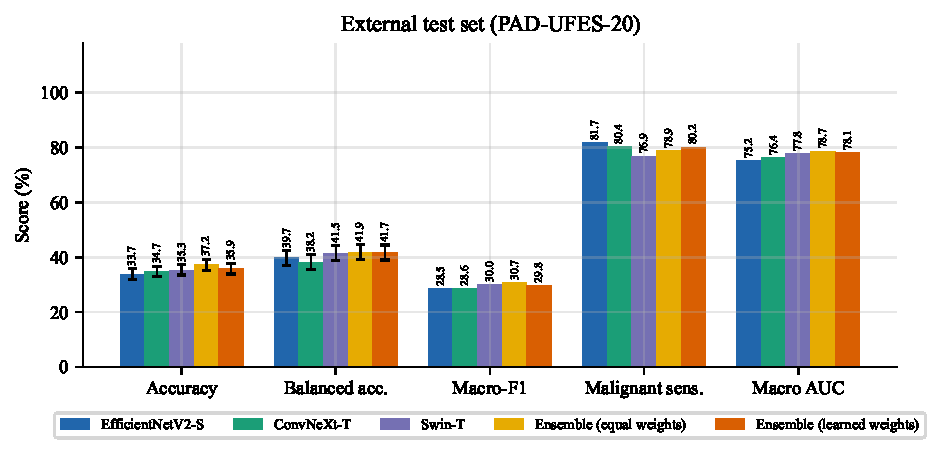
\includegraphics[width=\ifCLASSOPTIONtwocolumn0.80\textwidth\else\linewidth\fi]{figures/fig_external_comparison.pdf}\\[2pt]
{\footnotesize (b) External test set (PAD-UFES-20)}
\caption{Measured performance of the three single models and the two
ensembles. Error bars show 95\% bootstrap confidence intervals for
accuracy and balanced accuracy.}
\label{fig:comparison}
\ifCLASSOPTIONtwocolumn\end{figure*}\else\end{figure}\fi

\subsection{Per-Class Behaviour}
Fig.~\ref{fig:confusion} shows the confusion matrix of the equal-weight
ensemble with image counts, and Table~\ref{tab:perclass} gives
precision, recall, and F1 per class. Nevi (91.4\% recall, 86.4\%
precision), vascular lesions (81.0\%, 89.5\%), and BCC (79.6\%, 77.0\%)
were recognized best, followed by melanoma (65.8\%, 68.5\%). The hardest
classes were the rare ones: SCC (48.5\%, 39.3\%), AK (43.0\%, 38.5\%), and
dermatofibroma (39.0\% recall at 76.7\% precision). The errors are
clinically plausible. Melanomas were most often confused with nevi (159
of 641), AK and SCC with BCC (45 of 128 and 16 of 68), and
dermatofibromas with nevi (16 of 59). Fig.~\ref{fig:roc} shows that the ensemble also gives
the best malignant-versus-benign ROC curve (AUC 0.934 with equal
weights, against 0.910--0.926 for the single models).

\begin{figure}[t]
\centering
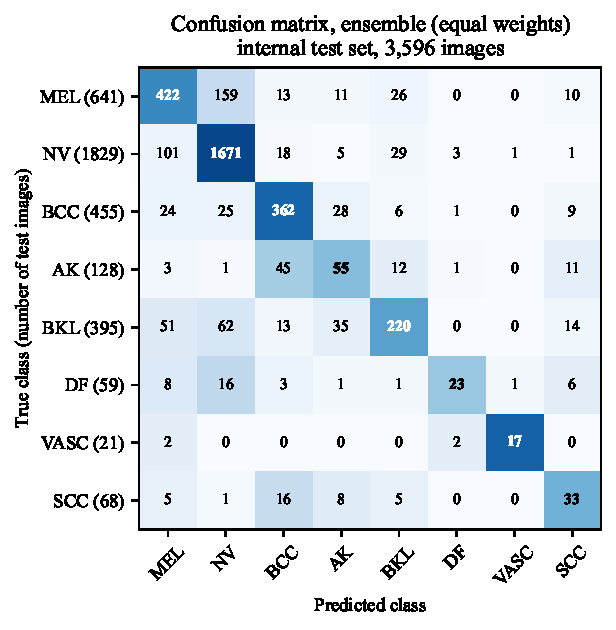
\includegraphics[width=0.95\columnwidth]{figures/fig_cm_counts.pdf}
\caption{Confusion matrix of the equal-weight ensemble on the internal
test set (number of images; diagonal = correct). Accuracy = sum of the
diagonal / all images = 2{,}803 / 3{,}596 = 77.95\%.}
\label{fig:confusion}
\end{figure}

\begin{table}[t]
\centering
\caption{Per-class precision, recall, and F1 (\%) of the equal-weight
ensemble on the internal test set.}
\label{tab:perclass}
\renewcommand{\arraystretch}{1.12}
\footnotesize
\begin{tabular}{@{}l r c c c@{}}
\toprule
\textbf{Class} & \textbf{Images} & \textbf{Precision} & \textbf{Recall} & \textbf{F1} \\
\midrule
Melanoma (MEL) & 641 & 68.5 & 65.8 & 67.1 \\
Nevus (NV) & 1{,}829 & 86.4 & 91.4 & 88.8 \\
BCC & 455 & 77.0 & 79.6 & 78.3 \\
Actinic keratosis (AK) & 128 & 38.5 & 43.0 & 40.6 \\
Benign keratosis (BKL) & 395 & 73.6 & 55.7 & 63.4 \\
Dermatofibroma (DF) & 59 & 76.7 & 39.0 & 51.7 \\
Vascular (VASC) & 21 & 89.5 & 81.0 & 85.0 \\
SCC & 68 & 39.3 & 48.5 & 43.4 \\
\midrule
Macro average & 3{,}596 & 68.7 & 63.0 & 64.8 \\
\bottomrule
\end{tabular}
\end{table}

\begin{figure}[t]
\centering
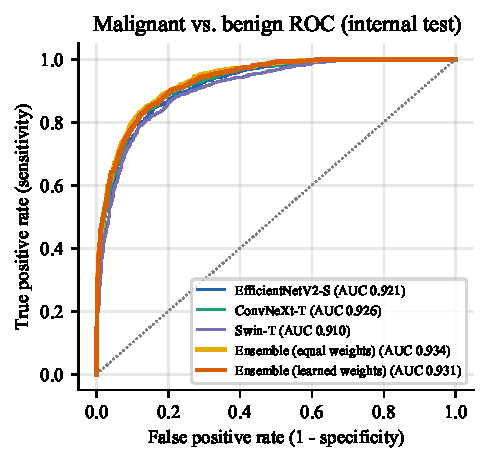
\includegraphics[width=0.88\columnwidth]{figures/fig_roc_malignant.pdf}
\caption{Malignant (MEL, BCC, SCC, AK) versus benign ROC curves on the
internal test set.}
\label{fig:roc}
\end{figure}

\subsection{Effect of Combining Models}
Table~\ref{tab:ablation} isolates the contribution of model combination.
Every pair of backbones beat each of its members, and the full
three-model ensemble beat every pair. Adding the transformer (Swin-T)
to the two CNNs raised balanced accuracy from 61.31\% to 62.99\% and the
external malignant AUC from 0.860 to 0.873, even though Swin-T was the
weakest single model. This supports the central idea of this work:
models with different inductive biases make different errors, and
combining them improves the result.

\begin{table}[t]
\centering
\caption{Ablation: effect of combining backbones (equal-weight soft
voting; measured). Int.\ = internal test, Ext.\ = PAD-UFES-20; Mal.\ AUC =
malignant-versus-benign AUC.}
\label{tab:ablation}
\renewcommand{\arraystretch}{1.12}
\footnotesize
\setlength{\tabcolsep}{3.5pt}
\begin{tabularx}{\columnwidth}{@{}Y c c c c@{}}
\toprule
\textbf{Models combined} & \textbf{Int.\ Acc.} & \textbf{Int.\ BA} & \textbf{Int.\ Mal.\ AUC} & \textbf{Ext.\ Mal.\ AUC} \\
\midrule
EffNetV2-S & 75.19 & 58.88 & 0.921 & 0.833 \\
ConvNeXt-T & 76.89 & 60.21 & 0.926 & 0.844 \\
Swin-T & 73.08 & 57.80 & 0.910 & 0.844 \\
\midrule
EffNetV2-S + ConvNeXt-T & 77.20 & 61.31 & 0.933 & 0.860 \\
EffNetV2-S + Swin-T & 76.70 & 62.39 & 0.928 & 0.864 \\
ConvNeXt-T + Swin-T & 77.09 & 61.55 & 0.929 & 0.866 \\
\midrule
\textbf{All three} & \textbf{77.95} & \textbf{62.99} & \textbf{0.934} & \textbf{0.873} \\
\bottomrule
\end{tabularx}
\end{table}

\subsection{External Test Set (PAD-UFES-20)}
Table~\ref{tab:res_external} and Fig.~\ref{fig:comparison}(b) show a
large drop on smartphone images. Accuracy fell to 33.7--37.3\% and
balanced accuracy to 38.2--41.9\% for all models. Per class, nevi (82\%
recall) and benign keratoses (68\%) still transferred reasonably, but
BCC (43\%), melanoma (37\%), AK (14\%), and SCC (8\%) did not. Two
factors explain this. First, PAD-UFES-20 consists of clinical photographs
taken with ordinary phones, whereas all training images are dermoscopic.
Second, its class mix differs strongly (37\% BCC and 32\% AK). The
ranking of lesions by malignancy is more robust than the eight-class
decision. Combining the three models raised the malignant-versus-benign
AUC from 0.833--0.844 (single models) to \textbf{0.873}. At the threshold
chosen on internal validation data, the ensemble detected 78.9\% of
malignant or pre-malignant lesions at 80.8\% specificity. These results
reproduce, with our own models, the benchmark-to-clinic gap documented
in the literature~\cite{menzies2023,tschandl2019comparison}.

\begin{table}[t]
\centering
\caption{Measured results on the external test set (PAD-UFES-20, 2{,}298
smartphone images, 6 shared classes).}
\label{tab:res_external}
\renewcommand{\arraystretch}{1.15}
\scriptsize
\setlength{\tabcolsep}{3pt}
\begin{tabular}{@{}l c c c c c c c@{}}
\toprule
\textbf{Model} & \textbf{Acc.} & \textbf{BA} & \textbf{Prec.} & \textbf{F1} & \textbf{AUC} & \textbf{Sens.} & \textbf{Spec.} \\
\midrule
EfficientNetV2-S & 33.68 & 39.74 & 34.75 & 28.50 & 0.752 & 81.7 & 68.5 \\
ConvNeXt-T & 34.73 & 38.22 & 33.82 & 28.64 & 0.764 & 80.4 & 74.3 \\
Swin-T & 35.34 & 41.50 & 35.34 & 30.03 & 0.778 & 76.9 & 75.6 \\
\textbf{Ensemble (equal)} & \textbf{37.25} & \textbf{41.89} & \textbf{37.05} & \textbf{30.74} & \textbf{0.787} & 78.9 & \textbf{80.8} \\
Ensemble (learned) & 35.86 & 41.72 & 35.75 & 29.78 & 0.781 & 80.2 & 77.2 \\
\bottomrule
\end{tabular}
\end{table}

\subsection{Skin-Type Analysis}
On PAD-UFES-20, the equal-weight ensemble reached a malignant AUC of
0.868 for Fitzpatrick types I--II (1{,}029 images) and 0.845 for types
III--IV (454 images), with similar accuracy (35.3\% and 36.3\%). Only 11
images belong to types V--VI, which is far too few for a reliable
estimate. This confirms the diversity gap reported in the
literature~\cite{wen2022} and is why the DDI dataset is planned as the
next fairness test.

% ================  VI. COMPARATIVE ANALYSIS OF ALGORITHMS  ===============
\section{Comparative Analysis of Algorithms}\label{sec:compare}
This section compares algorithm families using results reported in the
literature, and places our own measured result alongside them. Because
numbers from different protocols are not directly comparable, results are grouped into four protocol-consistent panels:
(A) HAM10000/ISIC~2018 seven-class with random splits,
(B) ISIC~2019 eight-class, (C) patient-disjoint HAM10000 with frozen
encoders, and (D) segmentation on ISIC~2018 under one re-implementation.
Table~\ref{tab:compare} lists all values with their protocol.

\begin{table*}[t]
\centering
\caption{Comparative analysis of algorithms for skin lesion classification and segmentation (values exactly as reported in each source).}
\label{tab:compare}
\renewcommand{\arraystretch}{1.13}
\scriptsize
\begin{tabularx}{\textwidth}{@{}c l l l l Y@{}}
\toprule
\textbf{Panel} & \textbf{Family} & \textbf{Model} & \textbf{Dataset (classes)} & \textbf{Reported result} & \textbf{Protocol / note} \\
\midrule
\multirow{11}{*}{A} & Classical ML & SVM~\cite{shetty2022} & HAM10000 subset (7) & Acc.\ 53\%, W-F1 0.50 & 100 img/class + aug., $k$-fold \\
 & Classical ML & Random forest~\cite{shetty2022} & HAM10000 subset (7) & Acc.\ 87\% & Same protocol as SVM \\
 & CNN & ResNet-50, CE loss~\cite{nie2023hybrid} & ISIC~2018 (7) & Acc.\ 74.2\% & Random 70/10/20 \\
 & CNN (light) & MobileNet~\cite{chaturvedi2020mobilenet} & HAM10000 (7) & Acc.\ 83.1\%, W-F1 0.83 & Random split \\
 & CNN & ResNet-50, focal loss~\cite{nie2023hybrid} & ISIC~2018 (7) & Acc.\ 83.7\% & Same split as CE row \\
 & CNN & EfficientNet-B4~\cite{ali2022efficientnets} & HAM10000 (7) & Acc.\ 87.9\%, F1 0.87 & Best of B0--B7 \\
 & Hybrid & ResNet + ViT, focal~\cite{nie2023hybrid} & ISIC~2018 (7) & Acc.\ 89.5\%, macro-F1 81.1\% & Same split as CE row \\
 & CNN & ResNeXt-101~\cite{chaturvedi2020mtap} & HAM10000 (7) & Acc.\ 93.2\% & Best of five CNNs \\
 & CNN + attention & InceptionResNetV2 + SA~\cite{datta2021soft} & HAM10000 (7) & Acc.\ 93.4\%, AUC 0.984 & Resampled random split \\
 & Hybrid & Swin + DenseNet attn.~\cite{karthik2024} & HAM10000 (7) & Acc.\ 94.2\% & Single dataset \\
 & Transformer & SkinTrans (ViT)~\cite{xin2022skintrans} & HAM10000 (7) & Acc.\ 94.3\% & Split not detailed \\
\midrule
\multirow{6}{*}{B} & CNN & EfficientNet-B0~\cite{gessert2020} & ISIC~2019 (8) & BA 65.8\% (67.4\% + meta) & 5-fold CV \\
 & Ensemble & Multi-res.\ EfficientNets + meta~\cite{gessert2020} & ISIC~2019 (8) & BA 74.2\% (CV) & 5-fold CV \\
 & Ensemble & same, official test~\cite{gessert2020} & ISIC~2019 (8+unk.) & BA 63.6\% & Hidden test with unknown class \\
 & Transformer & Swin~\cite{ayas2023swin} & ISIC~2019 (8) & BA 82.3\%, spec.\ 97.9\% & Hold-out split \\
 & Ensemble & ConvNeXt T/S/B/L~\cite{baykal2024convnext} & ISIC~2019 (8) & Sens.\ 84.2\%, spec.\ 97.9\% & Same group as Swin row \\
 & \textbf{Ensemble} & \textbf{EffNetV2-S + ConvNeXt-T + Swin-T (ours)} & ISIC~2019 (8) & \textbf{BA 63.0\%, acc.\ 78.0\%} & Lesion-disjoint held-out test, 224\,px \\
\midrule
\multirow{3}{*}{C} & ViT (ImageNet) & ViT-L linear probe~\cite{yan2025panderm} & HAM10000 clean (7) & BA 65.3\%, AUC 0.970 & Patient-disjoint 60/20/20 \\
 & Self-supervised & DINOv2 ViT-L probe~\cite{yan2025panderm} & HAM10000 clean (7) & BA 70.1\%, AUC 0.964 & Patient-disjoint \\
 & Foundation & PanDerm ViT-L probe~\cite{yan2025panderm} & HAM10000 clean (7) & BA 80.7\%, AUC 0.988 & Patient-disjoint \\
\midrule
\multirow{2}{*}{--} & Ensemble & EfficientNet ens.\ + meta~\cite{ha2020siim} & ISIC~2020 (2) & AUC 0.949 & Official private leaderboard \\
 & CNNs (19) & Best after de-dup.~\cite{cassidy2022isic} & ISIC~2020 (2) & AUC 0.80 & Duplicates removed \\
\midrule
\multirow{4}{*}{D} & CNN & U-Net~\cite{azad2024unet} & ISIC~2018 T1 & Dice 0.867, IoU 0.849 & Uniform re-run, 224 px \\
 & CNN + attention & Attention U-Net~\cite{azad2024unet} & ISIC~2018 T1 & Dice 0.882, IoU 0.865 & Same \\
 & Transformer & TransUNet~\cite{azad2024unet} & ISIC~2018 T1 & Dice 0.850, IoU 0.837 & Same \\
 & Hybrid & UCTransNet~\cite{azad2024unet} & ISIC~2018 T1 & Dice 0.890, IoU 0.873 & Same \\
\bottomrule
\end{tabularx}
\end{table*}

\subsection{Panel A: Seven-Class HAM10000 / ISIC~2018}
Fig.~\ref{fig:cmpA} ranks eleven algorithms. Deep models clearly
outperform the classical baselines, and within deep models the trend
moves from plain CNNs (74--88\%) through attention-augmented CNNs and
hybrids (89--94\%) to transformers (94\%). The most informative
comparison is the controlled one by Nie \emph{et al.}~\cite{nie2023hybrid}:
with backbone and split fixed, focal loss adds 9.5 points and the
hybrid transformer adds another 5.7. The \emph{training strategy} can
therefore matter as much as the architecture. Note that all Panel~A
results use image-level random splits, which are known to be
optimistic~\cite{cassidy2022isic}.

\begin{figure}[t]
\centering
\begin{tikzpicture}
\begin{axis}[hcaxis,
  width=\barchartw,height=\tallcharth,
  xbar, bar width=5.5pt, bar shift=0pt,
  ytick={1,...,11},
  legend style={at={(0.5,-0.22)},anchor=north,legend columns=3},
  yticklabels={SVM,Random forest,ResNet-50 (CE),MobileNet,ResNet-50 (focal),EfficientNet-B4,CNN+ViT hybrid,ResNeXt-101,IRv2 + attention,Swin+DenseNet,SkinTrans (ViT)},
  y tick label style={font=\scriptsize},
  xlabel={Reported accuracy (\%)},
  xmin=40,xmax=102, nodes near coords,
  every node near coord/.append style={font=\tiny},
  enlarge y limits=0.06]
\addplot[fill=hcGray,draw=hcGray!60] coordinates {(53,1)(87,2)};
\addplot[fill=hcBlue,draw=hcBlue!60] coordinates {(74.2,3)(83.1,4)(83.7,5)(87.9,6)(93.2,8)(93.4,9)};
\addplot[fill=hcPurple,draw=hcPurple!60] coordinates {(89.5,7)(94.2,10)(94.3,11)};
\legend{Classical ML,CNN,Transformer / hybrid}
\end{axis}
\end{tikzpicture}
\caption{Panel A: reported seven-class accuracy on HAM10000/ISIC~2018
(random splits) for classical, CNN, and transformer/hybrid algorithms
(sources in Table~\ref{tab:compare}).}
\label{fig:cmpA}
\end{figure}

\subsection{Panel B: Eight-Class ISIC~2019}
ISIC~2019 is harder: it adds SCC, has a larger and more heterogeneous
image pool, and is normally scored with balanced accuracy.
Fig.~\ref{fig:cmpB} shows two lessons. First, ensembles beat single
models (74.2\% vs.\ 65.8\% BA for Gessert \emph{et al.}), and modern
backbones (Swin, ConvNeXt) score higher still. Second, the same winning
ensemble dropped from 74.2\% in cross-validation to 63.6\% on the
official hidden test set, which also contains unseen ``unknown''
lesions. This ten-point drop is larger than the differences between most
architectures, and it is the main reason our protocol evaluates on
external data. Our ensemble reached 63.0\% balanced accuracy on a
lesion-disjoint held-out test set (orange bar). That is the same level as
the ISIC~2019 winner on the official test set (63.6\%), although the two
test sets differ and that system used higher resolutions and metadata.
It is clearly below the hold-out results reported for Swin and ConvNeXt
ensembles, whose split details were not reported.

\begin{figure}[t]
\centering
\begin{tikzpicture}
\begin{axis}[hcaxis,
  width=\chartw,height=\charth,
  ybar, bar width=10pt,
  xtick={1,...,7},
  xticklabels={EffNet-B0,EffNet-B0 +meta,Ensemble (CV),Ensemble (test),Swin,ConvNeXt ens.,Ours (test)},
  x tick label style={rotate=25,anchor=east,font=\tiny},
  bar shift=0pt,
  legend style={at={(0.5,1.02)},anchor=south,legend columns=2},
  ylabel={BA / mean sensitivity (\%)},
  ymin=50,ymax=92, nodes near coords,
  every node near coord/.append style={font=\tiny},
  enlarge x limits=0.1]
\addplot[fill=hcBlue,draw=hcBlue!60] coordinates {(1,65.8)(2,67.4)(3,74.2)(5,82.3)(6,84.2)};
\addplot[fill=hcRed,draw=hcRed!60] coordinates {(4,63.6)};
\addplot[fill=hcOrange,draw=hcOrange!60] coordinates {(7,63.0)};
\legend{Reported (validation),Reported (hidden test),Ours (held-out test)}
\end{axis}
\end{tikzpicture}
\caption{Panel B: ISIC~2019 eight-class balanced accuracy. The red bar
shows the ISIC~2019 winner on the official test set, 10.6 points below
its own cross-validation score~\cite{gessert2020,ayas2023swin,baykal2024convnext};
the orange bar is our measured ensemble on a lesion-disjoint test set.}
\label{fig:cmpB}
\end{figure}

\subsection{Panel C: Patient-Disjoint Evaluation of Pretraining}
Panel C is the fairest comparison, because all three encoders were
evaluated by the same authors with a patient-disjoint split and an
identical linear classifier~\cite{yan2025panderm}. Fig.~\ref{fig:cmpC}
shows that the \emph{pretraining source} changes balanced accuracy by
more than 15 points: ImageNet features reach 65.3\%, general
self-supervised DINOv2 features 70.1\%, and dermatology-specific PanDerm
features 80.7\%. AUC hides this difference (0.96--0.99), which again
argues for balanced accuracy as the primary metric.

\begin{figure}[t]
\centering
\begin{tikzpicture}
\begin{axis}[hcaxis,
  width=\chartw,height=\charth,
  ybar, bar width=11pt,
  symbolic x coords={ImageNet ViT-L,DINOv2 ViT-L,PanDerm ViT-L},
  xtick=data, x tick label style={font=\scriptsize},
  ylabel={Score (\%)},
  ymin=50,ymax=104, nodes near coords,
  every node near coord/.append style={font=\tiny},
  legend style={at={(0.5,1.02)},anchor=south,legend columns=3},
  enlarge x limits=0.25]
\addplot[fill=hcBlue,draw=hcBlue!60] coordinates {(ImageNet ViT-L,65.3)(DINOv2 ViT-L,70.1)(PanDerm ViT-L,80.7)};
\addplot[fill=hcTeal,draw=hcTeal!60] coordinates {(ImageNet ViT-L,87.9)(DINOv2 ViT-L,88.3)(PanDerm ViT-L,92.6)};
\addplot[fill=hcOrange,draw=hcOrange!60] coordinates {(ImageNet ViT-L,97.0)(DINOv2 ViT-L,96.4)(PanDerm ViT-L,98.8)};
\legend{Balanced acc.,Weighted F1,AUC}
\end{axis}
\end{tikzpicture}
\caption{Panel C: linear-probe results on a patient-disjoint HAM10000
split~\cite{yan2025panderm}. Domain-specific pretraining gives the
largest balanced-accuracy gain.}
\label{fig:cmpC}
\end{figure}

\subsection{Panel D: Lesion Segmentation}
Under a single uniform re-implementation on ISIC~2018~\cite{azad2024unet},
attention gates improve U-Net Dice from 0.867 to 0.882, and the hybrid
UCTransNet reaches 0.890, whereas the pure-transformer TransUNet is
lowest at 0.850 (Fig.~\ref{fig:cmpD}). With limited data, the
convolutional inductive bias still helps; this supports our choice of an
attention U-Net for the segmentation stage.

\begin{figure}[t]
\centering
\begin{tikzpicture}
\begin{axis}[hcaxis,
  width=\chartw,height=\charth,
  ybar, bar width=9pt,
  symbolic x coords={U-Net,Attention U-Net,TransUNet,UCTransNet},
  xtick=data, x tick label style={font=\scriptsize},
  ylabel={Score},
  ymin=0.80,ymax=0.91, nodes near coords,
  every node near coord/.append style={font=\tiny,/pgf/number format/fixed,/pgf/number format/precision=3},
  yticklabel style={/pgf/number format/fixed,/pgf/number format/precision=2},
  legend style={at={(0.5,1.02)},anchor=south,legend columns=2},
  enlarge x limits=0.18]
\addplot[fill=hcTeal,draw=hcTeal!60] coordinates {(U-Net,0.8674)(Attention U-Net,0.8820)(TransUNet,0.8499)(UCTransNet,0.8898)};
\addplot[fill=hcPurple,draw=hcPurple!60] coordinates {(U-Net,0.8491)(Attention U-Net,0.8649)(TransUNet,0.8365)(UCTransNet,0.8729)};
\legend{Dice,IoU}
\end{axis}
\end{tikzpicture}
\caption{Panel D: segmentation performance on ISIC~2018 Task~1 under a
uniform protocol~\cite{azad2024unet}.}
\label{fig:cmpD}
\end{figure}

\subsection{Benchmark versus Clinic}
Fig.~\ref{fig:clinic} compares sensitivity and specificity from three
prospective studies. All AI systems operate at high sensitivity but
with specificities of 28--67\%, which would generate many unnecessary
referrals or biopsies. Dermatologists in the same multicentre study had
lower sensitivity but much higher specificity~\cite{heinlein2024}. These
findings motivate the explicit, validated operating threshold and
calibration step in our method.

\begin{figure}[t]
\centering
\begin{tikzpicture}
\begin{axis}[hcaxis,
  width=\chartw,height=\charth,
  ybar, bar width=7pt,
  xtick={1,...,5},
  xticklabels={PROVE-AI,DERM (SCC),DERM (BCC),AI (Heinlein),Dermatologists},
  x tick label style={rotate=20,anchor=east,font=\tiny},
  ylabel={\%}, ymin=0,ymax=112, nodes near coords,
  every node near coord/.append style={font=\tiny},
  legend style={at={(0.5,1.02)},anchor=south,legend columns=2},
  enlarge x limits=0.12]
\addplot[fill=hcTeal,draw=hcTeal!60] coordinates {(1,96.8)(2,98)(3,94)(4,92.1)(5,73.4)};
\addplot[fill=hcOrange,draw=hcOrange!60] coordinates {(1,37.4)(2,38)(3,28)(4,67.3)(5,82.8)};
\legend{Sensitivity,Specificity}
\end{axis}
\end{tikzpicture}
\caption{Prospective clinical performance: AI systems achieve high
sensitivity at low specificity~\cite{marchetti2023,marsden2023,heinlein2024}.}
\label{fig:clinic}
\end{figure}

\subsection{Qualitative Comparison of Algorithm Families}
Table~\ref{tab:qual} summarizes the trade-offs between families,
including approximate model size, which determines whether a model can
run on a phone or needs a server.

\begin{table*}[t]
\centering
\caption{Qualitative comparison of algorithm families for skin cancer detection (parameter counts are those of the standard ImageNet models).}
\label{tab:qual}
\renewcommand{\arraystretch}{1.15}
\scriptsize
\begin{tabularx}{\textwidth}{@{}l l c L{3.3cm} Y c@{}}
\toprule
\textbf{Family} & \textbf{Representative} & \textbf{Params} & \textbf{Strengths} & \textbf{Weaknesses} & \textbf{Used here} \\
\midrule
Classical ML & SVM, random forest & $<$1M & Fast, interpretable features & Far lower accuracy; handcrafted features & Baseline only \\
Plain CNN & VGG16 / ResNet-50 & 138M / 25.6M & Mature, easy transfer learning & VGG is heavy; limited global context & Baseline \\
Dense / Inception CNN & DenseNet-121, InceptionV3 & 8.0M / 23.8M & Feature reuse; multi-scale filters & Moderate accuracy on ISIC~2019 & Baseline \\
Lightweight CNN & MobileNetV2 & 3.5M & Runs on smartphones & Lower accuracy on rare classes & Baseline, future distillation \\
Scaled CNN & EfficientNet / V2-S & 5.3M--22M & Best accuracy per FLOP; challenge winner & Sensitive to input resolution & \checkmark \\
Modern CNN & ConvNeXt-T & 28M & Transformer-style design, CNN efficiency & Needs strong augmentation & \checkmark \\
Vision transformer & ViT-B/16 & 86M & Global attention & Data-hungry; weak with small data & Probe baseline \\
Hierarchical transformer & Swin-T & 28M & Global + local windows; strong on ISIC~2019 & Higher memory at high resolution & \checkmark \\
Hybrid CNN--ViT & ResNet+ViT, Swin+DenseNet & varies & Complementary local/global features & More complex; rarely externally tested & Ensemble design \\
Ensemble & Multi-backbone voting & Sum of members & Most robust; wins challenges & Slower inference & \checkmark \\
Foundation model & PanDerm, DINOv2 & 300M+ & Best transfer, label-efficient & Heavy compute; licence constraints & Future work \\
\bottomrule
\end{tabularx}
\end{table*}

% ==========================  VII. DISCUSSION  ==========================
\section{Discussion}\label{sec:discuss}
\textbf{Main findings.} The comparative analysis supports four
conclusions. (i) Deep learning clearly outperforms classical machine
learning for skin cancer detection. (ii) Among deep models, ensembles
and CNN--transformer combinations are consistently the strongest, but
the margins between modern backbones are only a few points. (iii)
Evaluation choices---random versus grouped splits, internal versus
external data, accuracy versus balanced accuracy---shift results by
10--15 points, more than the architecture does. (iv) Imbalance handling
and domain-specific pretraining are the two cheapest sources of large
gains. Our own experiments confirm the second and third points. The
three-model ensemble outperformed every single model and every pair on
internal data (77.95\% accuracy, 62.99\% balanced accuracy). The same
models lost about 40 points of accuracy on external smartphone images,
far more than the fewer than 4 points that separate the backbones.

\textbf{Why not claim 99\% accuracy?} Several recent papers report
97--100\% accuracy on HAM10000~\cite{naeem2025,behara2023}. Without
patient-level splits and external tests, such numbers mainly reflect
near-duplicate images. We therefore set our success criteria on
external and per-skin-tone performance rather than on internal
accuracy.

\textbf{Why does the ensemble help?} The single models make partly
different errors. For example, Swin-T had the best AK recall (50\%) but
the worst BCC recall (65\%), while ConvNeXt-T showed the opposite
pattern. Averaging calibrated probabilities therefore corrects some
errors of each member. It also improves specificity at a fixed
sensitivity, which matters for referral. The gains are consistent but
modest (about 1--3 points of balanced accuracy), and the confidence
intervals of the best single model and the ensemble overlap. A larger
test set or repeated splits are needed to confirm the size of the
improvement.

\textbf{Limitations.} The reported experiments use one lesion-grouped
split, $224\times224$ inputs, and whole images. Segmentation, metadata
fusion, colour constancy, and Grad-CAM are not yet included, and the
weights learned on validation data did not beat simple averaging. The
external accuracy on smartphone images is low, so the current models
must not be used on such images without domain adaptation or
fine-tuning on clinical photographs. Published numbers in
Table~\ref{tab:compare} come from different authors and are comparable
only within a panel. Only 11 external images come from Fitzpatrick types
V--VI, so fairness for darker skin remains untested. The system is intended as a
decision-support tool for clinicians, not an autonomous diagnostic
device. Clinical use would require prospective validation and
regulatory approval.

\textbf{Ethics.} Only de-identified public datasets are used, under
their respective licences (mostly CC BY-NC). The model will be
released with a model card that lists per-skin-tone performance and
known failure modes.

% ==========================  VIII. CONCLUSION  =========================
\section{Conclusion and Future Work}\label{sec:conc}
This paper reviewed deep learning for skin cancer detection, analysed
eleven public datasets, and compared classical, CNN, transformer,
hybrid, ensemble, foundation, and segmentation models using published
results grouped by comparable protocol. The comparison shows that
ensembles of complementary CNN and transformer backbones, trained with
imbalance-aware losses and metadata, are the most effective practical
choice. It also shows that leakage-free and external evaluation matter
more than any single architecture. Building on these findings, we
trained two CNNs (EfficientNetV2-S, ConvNeXt-T) and a transformer
(Swin-T) on ISIC~2019 with focal loss and a leakage-free split, and
combined them by calibrated soft voting. On 3{,}596 held-out images the
ensemble achieved \textbf{77.95\% accuracy}, \textbf{62.99\% balanced
accuracy}, a macro-AUC of \textbf{0.950}, and \textbf{95.4\%} malignant
sensitivity at 69.9\% specificity, outperforming every single model and
every pair of models. On the external smartphone dataset PAD-UFES-20,
accuracy dropped to 37.25\%, but the ensemble still gave the best
malignant-versus-benign AUC (0.873). Combining multiple algorithms
is therefore a reliable way to improve skin cancer detection, while
transfer to new imaging conditions remains the main open problem.
Future work will (1) add the segmentation, metadata, and Grad-CAM
modules and measure their contribution, (2) train at higher resolution
and fine-tune on clinical and smartphone images (PAD-UFES-20, MILK10k)
to close the domain gap, (3) evaluate fairness on DDI, (4) distil the
ensemble into a MobileNet-class student for smartphone use, and (5)
explore dermatology foundation-model features.

% =========================  REFERENCES  ==============================
\ifCLASSOPTIONtwocolumn\balance\fi
\bibliographystyle{IEEEtran}
\bibliography{references}
